% Preamble. Don't worry about it.
\documentclass{article}
\usepackage{setspace,graphicx,fancyhdr}
\usepackage[utf8]{inputenc}
\usepackage[left=1in,top=1in,right=1in,bottom=1in]{geometry} % Document margins
\onehalfspacing

% For custom footers
\pagestyle{fancy}
\fancyhead{}                        % clear all header fields
\renewcommand{\headrulewidth}{0pt}  % no line in header area
\fancyfoot{}                        % clear all footer fields
\fancyfoot[LE,RO]{\thepage}         % for page #s
\fancyfoot[RE,LO]{
\includegraphics{../images/logo/markshark-1x}}

% Setting the depth for Table of Contents
\setcounter{tocdepth}{2}

\begin{document}

% --- TITLE PAGE ---
\title{Donnervögel Consulting \\ MarkShark Grading System \\ Design Document}
\author{\textbf{Phase Lead: Stephen Laboucane}}
\maketitle
\centerline{
\includegraphics{../images/logo/markshark-10x}}
\clearpage
% ------------------

% --- REVISION HISTORY ---
\textbf{Revision History}
\begin{center}
  \begin{tabular}{| c | c | c | l |}
    \hline
    Version & Date & Members & Changes\\
    \hline
    1.0 & 2014 Mar 28 (Fri) & Stephen L. & Document created.\\
    & & Graeme S. & \\
    & & Colin W. &\\
    \hline
  \end{tabular}
\end{center}
\clearpage
% ------------------------

% --- TABLE OF CONTENTS ---
\tableofcontents
\clearpage
% -------------------------

\section{White Box} 
\subsection{Purpose}
% Describe the purpose of the method
\textit{loginButtonActionPerformed( )} in the LoginScreen class is called when the user clicks the login button on the login screen.  It takes the form data, and checks whether it is valid.  If true, then display the proper home page for the current user role.

\subsection{Code}
% Analyze the code for the method and break it into appropriate numbered blocks
\begin{verbatim}
private void loginButtonActionPerformed(ActionEvent evt) {
===============================================================================
1
    String name = username_field.getText();
    String pass = new String(pass_field.getPassword());
    Account test;
===============================================================================
2
    if(pass.length() < 0) 
===============================================================================
3
    {  // Temporary! Should be 5 or so.
        JOptionPane.showMessageDialog(this, "The password given is too short.");
    }
===============================================================================
4
    else if(name.isEmpty())
===============================================================================
5
    {
        JOptionPane.showMessageDialog(this, "No user name given.");
    }
===============================================================================
6
    else if(test == null) 
===============================================================================
7
    {
    	JOptionPane.showMessageDialog(this, "Invalid username/password combo");
    }
===============================================================================
8
    else
    {
        System.out.println("Logging in as " + name +
    		       " with password `" + pass + "`");
        // TODO: This needs to be passed a legit Account object.
        master = new MasterFrame(test);
        this.setVisible(false);
        master.run();
    }
===============================================================================
}
\end{verbatim}

\subsection{Flow Chart}
% Develop a flow chart for your method based on the blocks of code the method was broken into in the previous step
\centerline{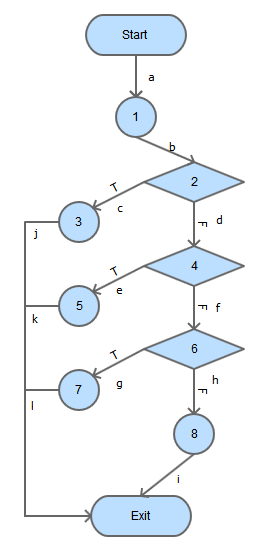
\includegraphics[scale=1.1]{../images/Whitebox_Testing_Diagram}}

\subsection{Coverage}
% Comment on the types of coverage needed to test the method
Statement coverage is sufficient, because all blocks have exactly one input branch, except for Exit.  All blocks one level above Exit have only one output branch (leading to Exit) so all paths through those blocks cover all paths to Exit.  In this way, branch testing is redundant.  Additionally, there are no loops, so a block can be executed at most once in a case.  As all branches have been covered, this would be unnecessary as well.

\subsection{List of Test Cases}
% Develop a list of test cases that will adequately test the method. Do not fully develop each test case. ONLY list the coverage of each test and explain why the test is needed/useful
\begin{center}
  \begin{tabular}{| c | l |}
    \hline
    ID & Coverage\\
    \hline
    1S & START-1-2-3-EXIT\\
    2S & START-1-2-4-5-EXIT\\
    3S & START-1-2-4-6-7-EXIT\\
    4S & START-1-2-4-6-8-EXIT\\
    \hline
  \end{tabular}
\end{center}

\subsection{Detailed Test Case}
% Choose one of the test cases and describe it in detail in terms of the test case format used in class \\
% Demonstrate how your selected test case (input values) will help test the intended coverage.
\subsubsection{Test ID}
3S

\subsubsection{Test Purpose}
Unit test method \textit{loginButtonActionPerformed( )} of the LoginScreen class using White Box testing strategy (statement coverage: START-1-2-4-6-7-EXIT)

\subsubsection{Requirement Number}
\#

\subsubsection{Testing Procedure}
% >
Enter a username and password both of length > 5, "username" and "password".  Click the Log in button.

\subsubsection{Evaluation}
% How to evaulate it.  I don't think anything happens.
Login denied.

\subsubsection{Expected Behaviours and Results}
An error message should pop up saying "Invalid username/password combo," the user should still be on the login page, and therefore not be logged into the system.

\subsubsection{Actual Behavious and Results}
% May not print <> correctly.  Try changing encoding.
<Added at test time>

\section{Black Box}
\subsection{Purpose}
% Describe the purpose of the method, its parameters (arguments), and any preconditions necessary for successful execution of the method
\textit{execQuery(String) : ResultSet} executes an SQL query provided as the String argument, and returns the ResultSet storing the query's response.  The database connection details are defined in another function; they currently require the program to be run on the the Server's local network.  The database also must be operational.

\subsection{Equivalence Classes}
Describe the equivalence classes for each of the inputs and preconditions of this method

\subsection{Choosing Inputs}
% Describe how you would choose representative input values to test this method
Input values would come from valid and invalid equivalence classes.  Many of these are binary, so they would not have a boundary value to input.  Should test breaking preconditions with values from all valid equivalence classes, along with a set of all invalid equivalence class values, to make sure the preconditions are correct.

\subsection{List of Test Cases}
% Briefly describe how you would use the representative values to construct a set of test cases to test the method. DO NOT develop these test cases beyond describing them in terms of the values of the parameters and the preconditions.
\begin{center}
  \begin{tabular}{| c | l | l | l |}
    \hline
    ID & On Local Network & Server Status & SQL\\
    \hline
    1 & No & Not running & Valid\\
    2 & No & Running & Valid\\
	3 & Yes & Not running & Valid\\
    4 & Yes & Running & Invalid\\
    5 & Yes & Running & Valid\\
    6 & Yes & Running & Read permission denied\\
    7 & Yes & Running & Write permission denied\\
    8 & Yes & Running & Table does not exist\\
    9 & Yes & Running & Incorrect key\\
    10 & Yes & Running & Record does not exist\\
    11 & Yes & Running & Null\\
    12 & Yes & Running & Returns 0 tuples\\
    13 & Yes & Running & Returns 1 tuple of degree 1\\
    14 & Yes & Running & Returns 1 tuple of degree *\\
    15 & Yes & Running & Returns many tuples of degree 1\\
    16 & Yes & Running & Returns many tuples of degree *\\
    17 & Yes & Running & tuples contain null values\\
    \hline
  \end{tabular}
\end{center}

\subsection{Detailed Test Case}
% Select a single test case from those discussed in the previous item\\
% Describe your test case using the test case format seen in class.
\subsubsection{Test ID}
14

\subsubsection{Test Purpose}
Unit test CourseAccess class method \textit{execQuery( )} using Black box testing strategy

\subsubsection{Requirement Number}
\#

\subsubsection{Inputs}
\begin{itemize}
\item System is on the database's network
\item Database is operational
\item String = "SELECT * FROM c275g01A.dbo.Account WHERE Username = 'jtoering'"
\end{itemize}

\subsubsection{Testing Procedure}
Call \textit{execQuery}("SELECT * FROM c275g01A.dbo.Account WHERE Username = 'jToering'")

\subsubsection{Evaluation}
\begin{verbatim}
private static void testExecQueryWithAccount( ){
	ResultSet result={execQuery}("SELECT * FROM c275g01A.dbo.Account WHERE Username = 'jtoering'");
	try {
    	result.next();
	    System.out.println(result.getNString(1));
    	System.out.println(result.getNString(2));
	    System.out.println(result.getInt(3));
	    System.out.println(result.getNString(4));
	    System.out.println(int type=result.getInt(5));
	    } catch (SQLException ex) {
    	    System.out.println("SQL Exception occured, the state : "
                + ex.getSQLState() + "\nMessage: " + ex.getMessage());
        }
}
\end{verbatim}

\subsubsection{Expected Behaviours and Results}
\begin{verbatim}
jtoering
61843
99999
Jordan Toering
4
0
\end{verbatim}

\subsubsection{Actual Behaviours and Results}
% May not print <> correctly.  Try changing encoding.
<Added at test time>

\end{document}

% Fix <>'s
% Get Requirement #'s 1.6.3, 2.5.3
% Draw up equivalence classes 2.2
